%% This file was auto-generated by IPython, do NOT edit
%% Conversion from the original notebook file:
%% 03_Scaling_Python.ipynb
%%
\documentclass[11pt,english]{article}

%% This is the automatic preamble used by IPython.  Note that it does *not*
%% include a documentclass declaration, that is added at runtime to the overall
%% document.

\usepackage{amsmath}
\usepackage{amssymb}
\usepackage{graphicx}
\usepackage{ucs}
\usepackage[utf8x]{inputenc}
\usepackage{ctable}

% needed for markdown enumerations to work
\usepackage{enumerate}

% Slightly bigger margins than the latex defaults
\usepackage{geometry}
\geometry{verbose,tmargin=3cm,bmargin=3cm,lmargin=2.5cm,rmargin=2.5cm}

% Define a few colors for use in code, links and cell shading
\usepackage{color}
\definecolor{orange}{cmyk}{0,0.4,0.8,0.2}
\definecolor{darkorange}{rgb}{.71,0.21,0.01}
\definecolor{darkgreen}{rgb}{.12,.54,.11}
\definecolor{myteal}{rgb}{.26, .44, .56}
\definecolor{gray}{gray}{0.45}
\definecolor{lightgray}{gray}{.95}
\definecolor{mediumgray}{gray}{.8}
\definecolor{inputbackground}{rgb}{.95, .95, .85}
\definecolor{outputbackground}{rgb}{.95, .95, .95}
\definecolor{traceback}{rgb}{1, .95, .95}

% Framed environments for code cells (inputs, outputs, errors, ...).  The
% various uses of \unskip (or not) at the end were fine-tuned by hand, so don't
% randomly change them unless you're sure of the effect it will have.
\usepackage{framed}

% remove extraneous vertical space in boxes
\setlength\fboxsep{0pt}

% codecell is the whole input+output set of blocks that a Code cell can
% generate.

% TODO: unfortunately, it seems that using a framed codecell environment breaks
% the ability of the frames inside of it to be broken across pages.  This
% causes at least the problem of having lots of empty space at the bottom of
% pages as new frames are moved to the next page, and if a single frame is too
% long to fit on a page, will completely stop latex from compiling the
% document.  So unless we figure out a solution to this, we'll have to instead
% leave the codecell env. as empty.  I'm keeping the original codecell
% definition here (a thin vertical bar) for reference, in case we find a
% solution to the page break issue.

%% \newenvironment{codecell}{%
%%     \def\FrameCommand{\color{mediumgray} \vrule width 1pt \hspace{5pt}}%
%%    \MakeFramed{\vspace{-0.5em}}}
%%  {\unskip\endMakeFramed}

% For now, make this a no-op...
\newenvironment{codecell}{}

 \newenvironment{codeinput}{%
   \def\FrameCommand{\colorbox{inputbackground}}%
   \MakeFramed{\advance\hsize-\width \FrameRestore}}
 {\unskip\endMakeFramed}

\newenvironment{codeoutput}{%
   \def\FrameCommand{\colorbox{outputbackground}}%
   \vspace{-1.4em}
   \MakeFramed{\advance\hsize-\width \FrameRestore}}
 {\unskip\medskip\endMakeFramed}

\newenvironment{traceback}{%
   \def\FrameCommand{\colorbox{traceback}}%
   \MakeFramed{\advance\hsize-\width \FrameRestore}}
 {\endMakeFramed}

% Use and configure listings package for nicely formatted code
\usepackage{listingsutf8}
\lstset{
  language=python,
  inputencoding=utf8x,
  extendedchars=\true,
  aboveskip=\smallskipamount,
  belowskip=\smallskipamount,
  xleftmargin=2mm,
  breaklines=true,
  basicstyle=\small \ttfamily,
  showstringspaces=false,
  keywordstyle=\color{blue}\bfseries,
  commentstyle=\color{myteal},
  stringstyle=\color{darkgreen},
  identifierstyle=\color{darkorange},
  columns=fullflexible,  % tighter character kerning, like verb
}

% The hyperref package gives us a pdf with properly built
% internal navigation ('pdf bookmarks' for the table of contents,
% internal cross-reference links, web links for URLs, etc.)
\usepackage{hyperref}
\hypersetup{
  breaklinks=true,  % so long urls are correctly broken across lines
  colorlinks=true,
  urlcolor=blue,
  linkcolor=darkorange,
  citecolor=darkgreen,
  }

% hardcode size of all verbatim environments to be a bit smaller
\makeatletter 
\g@addto@macro\@verbatim\small\topsep=0.5em\partopsep=0pt
\makeatother 

% Prevent overflowing lines due to urls and other hard-to-break entities.
\sloppy

\begin{document}

\section{Python in HPC}


\subsection{Supercomputing 2012}

Presenters:


\noindent {\bf Andy R. Terrel, PhD}\\
Texas Advanced Computing Center\\
University of
Texas at Austin\\[2em]

\noindent {\bf Travis Oliphant, PhD}\\
Continuum Analytics\\[2em]

\noindent {\bf Aron Ahmadia, PhD}\\
Supercomputing Laboratory\\
King Abdullah University of Science and Technoglogy\\[2em]
\begin{center}

\href{http://creativecommons.org/licenses/by/3.0/deed.en\_US}{
\includegraphics{figures/creative_commons_logo.png}}\\[2em]

\noindent Python in HPC Tutorial by Terrel, Oliphant, and Ahmadia is licensed
under a Creative Commons Attribution 3.0 Unported License. \\[2em]

\href{http://www.tacc.utexas.edu}{
\includegraphics[scale=0.8]{figures/TACC_logo.png}} \qquad
\href{http://www.continuum.io}{
\includegraphics[scale=.3]{figures/continuum.png}} \qquad
\href{http://www.kaust.edu.sa/}{
\includegraphics[scale=.3]{figures/kaust.png}}
\end{center}

\newpage

\subsection{Updated Tutorial}

These presentation materials are being continuously updated as we refine
and improve our demonstrats. To get the latest version of this tutorial
you can:

\begin{enumerate}[1)]
\item
  Download a zip or tar ball from the
  \href{https://github.com/aterrel/HPCPythonSC2012/tags}{github SC2012
  tag}:

  wget --no-check-certificate
  https://github.com/aterrel/HPCPythonSC2012/zipball/SC2012
\item
  Checkout from git

  git clone https://github.com/aterrel/HPCPythonSC2012.git
\item
  View the html version on
  \href{http://nbviewer.ipython.org/urls/raw.github.com/aterrel/HPCPythonSC2012/master/03_Scaling_Python.ipynb}{nbviewer}.
\item
  As a last resort, head to https://github.com/aterrel/HPCPythonSC2012
  for updated instructions (see the README at the bottom of the page).
\end{enumerate}

\newpage

\subsection{Interacting with the Tutorial Slides}

This tutorial is an interactive worksheet designed to encourage you to
try out the lessons during the demonstration. If you are looking at the
pdf version, we encourage you to download the updated version (see
previous slide) and try the interactive version.

To run the interactive version, you need a good Python environment
including:

\begin{itemize}
\item
  IPython version \textgreater{}= 13.0
\item
  Numpy version \textgreater{}= 1.5
\item
  Scipy
\item
  Matplotlib
\end{itemize}

Move to the directory containing the tarball and execute:

\begin{verbatim}
$ ipython notebook --pylab=inline
\end{verbatim}

We heartily endorse the
\href{http://www.enthought.com/products/epd\_free.php}{Free Enthought
Python Distribution}.

\newpage
\subsection{Acknowledgements}

\begin{itemize}
\item
  Much of this tutorial adapts slide material from
  \href{http://www.cs.uiuc.edu/~wgropp/}{William Gropp}, University of
  Illinois
\item
  \href{http://code.google.com/p/mpi4py/}{mpi4py} is a
  \href{http://www.cython.org/}{Cythonized} wrapper around
  \href{http://www.mpi-forum.org/}{MPI} originally developed by
  \href{http://plus.google.com/107621373684536061961/about}{Lisandro
  Dalcin}, CONICET
\end{itemize}

\newpage
\subsection{The Free Lunch is Over}

\begin{figure}[htbp]
\centering
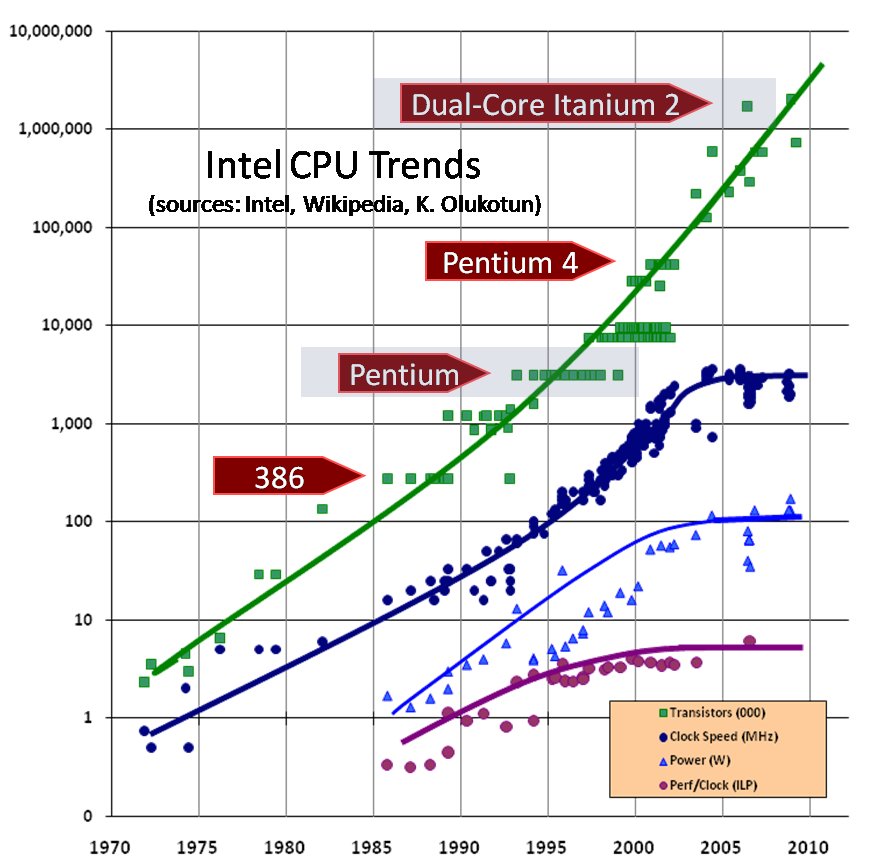
\includegraphics{figures/free_lunch.png}
\caption{freelunch}
\end{figure}

\newpage
\section{The Multiple Forms of Parallelism}

\begin{itemize}
\item
  \textbf{instruction} - multiple program instructions are
  simultaneously dispatched in a pipeline or to multiple execution units
  (superscalar)
\item
  \textbf{data} - the same program instructions are carried out
  simultaneously on multiple data items (SIMD)
\item
  \textbf{task} - different program instructions on different data
  (MIMD)
\item
  \textbf{collective} - single program, multiple data, not necessarily
  synchronized at individual operation level (SPMD)
\end{itemize}

\newpage
\subsection{The Rise of Manycore}

\begin{figure}[htbp]
\centering
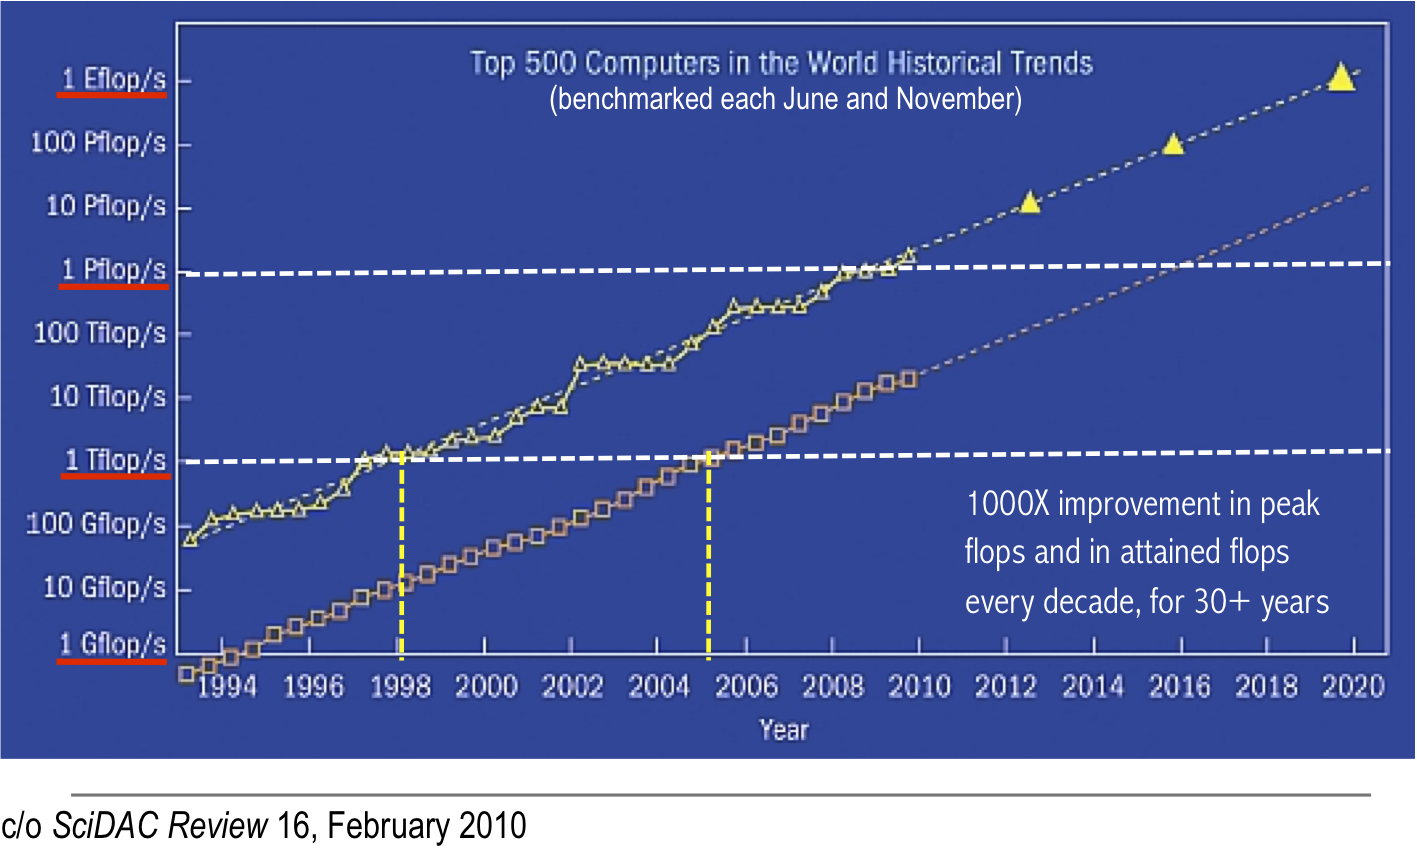
\includegraphics[scale=.75]{figures/concurrency_2.png}
\caption{Rise of Manycore}
\end{figure}

\newpage
\section{Parallel Architectures}

\begin{itemize}
\item
  All modern supercomputing architectures are composed of distributed
  memory compute nodes connected over toroidal networks
\item
  close mapping to physically n-dimensional problems
\item
  efficient algorithms exist for local point-to-point and collective
  communications across toroids
\item
  We expect to see higher dimensional interconnects and power-efficient
  networks that consume less power when not sending traffic
\end{itemize}

\newpage
\section{Parallel Programming Paradigms}

\begin{itemize}
\item
  a parallel programming paradigm is a specific approach to exploiting
  parallelism in hardware
\item
  many programming paradigms are very tightly coupled to the hardware
  beneath!
\item
  CUDA assumes large register files, Same Instruction Multiple Thread
  parallelism, and a mostly flat, structured memory model, matching the
  underlying GPU hardware
\item
  OpenMP exposes loop level parallelism with a fork/join model, assumes
  the presence of shared memory and atomics
\item
  OpenCl tries to generalize CUDA, but still assumes a `coprocessor'
  approach, where kernels are shipped from a master core to worker cores
\end{itemize}

\newpage
\subsection{The Message Passing Model}

\begin{itemize}
\item
  a process is (traditionally) a program counter for instructions and an
  address space for data
\item
  processes may have multiple threads (program counters and associated
  stacks) sharing a single address space
\item
  message passing is for communication among processes, which have
  separate address spaces
\item
  interprocess communication consists of
\item
  synchronization
\item
  movement of data from one process's address space to another's
\end{itemize}

\newpage
\subsection{Why MPI?}

\begin{itemize}
\item
  \textbf{communicators} encapsulate communication spaces for library
  safety
\item
  \textbf{datatypes} reduce copying costs and permit heterogeneity
\item
  multiple \textbf{communication modes} allow more control of memory
  buffer management
\item
  extensive \textbf{collective operations} for scalable global
  communication
\item
  \textbf{process topologies} permit efficient process placement, user
  views of process layout
\item
  \textbf{profiling interface} encourages portable tools
\end{itemize}

It Scales!

\newpage
\subsection{Python + MPI Does It Scale?}

\begin{itemize}
\item
  This and next slide courtesy the \textbf{PyClaw} project:
  http://numerics.kaust.edu.sa/pyclaw/
\item
  See also \textbf{GPAW}: https://wiki.fysik.dtu.dk/gpaw/
\end{itemize}

\begin{figure}[htbp]
\centering
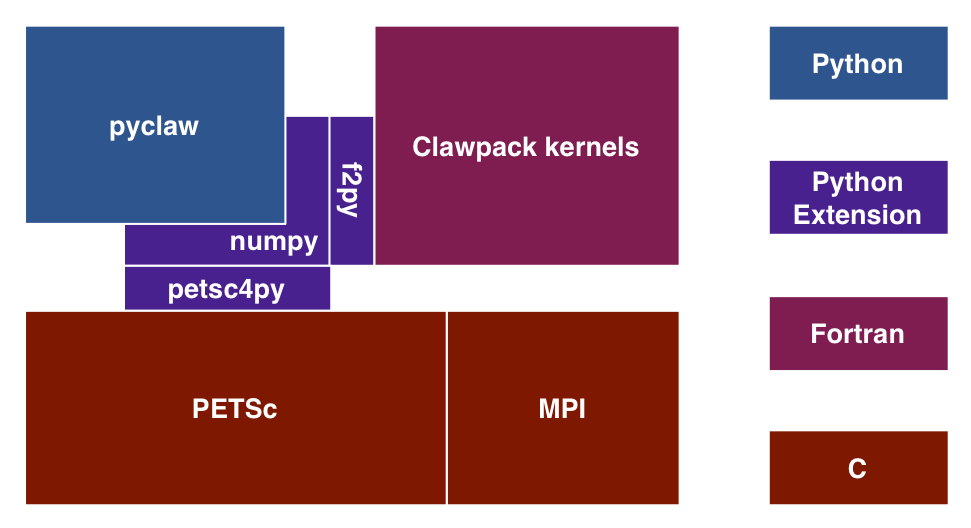
\includegraphics{figures/does_it_scale.png}
\caption{PyClaw Architecture}
\end{figure}

\newpage
\subsection{The Scalability of Python + MPI}

\begin{figure}[htbp]
\centering
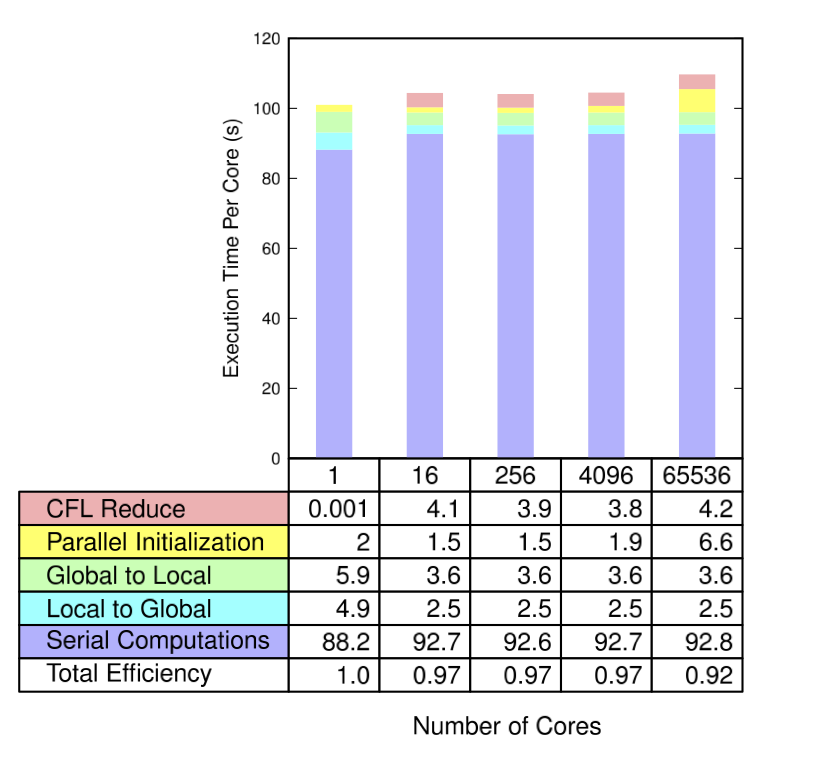
\includegraphics{figures/euler_weak_scaling.png}
\caption{Scalability}
\end{figure}

\newpage
\subsection{MPI - Quick Review}

\begin{itemize}
\item
  processes can be collected into \textbf{groups}
\item
  each message is sent in a \textbf{context}, and must be received in
  the same context
\item
  a \textbf{communicator} encapsulates a context for a specific group
\item
  a given program may have many communicators with any level of overlap
\item
  two initial communicators
\item
  \texttt{MPI\_COMM\_WORLD} (all processes)
\item
  \texttt{MPI\_COMM\_SELF} (current process)
\end{itemize}

\newpage
\subsection{Communicators}

\begin{itemize}
\item
  processes can be collected into \textbf{groups}
\item
  each message is sent in a \textbf{context}, and must be received in
  the same context
\item
  a \textbf{communicator} encapsulates a context for a specific group
\item
  a given program may have many communicators with any level of overlap
\item
  two initial communicators
\item
  \texttt{MPI\_COMM\_WORLD} (all processes)
\item
  \texttt{MPI\_COMM\_SELF} (current process)
\end{itemize}

\newpage
\subsection{Datatypes}

\begin{itemize}
\item
  the data in a message to send or receive is described by address,
  count and datatype
\item
  a datatype is recursively defined as:
\item
  predefined, corresponding to a data type from the language (e.g.,
  \texttt{MPI\_INT}, \texttt{MPI\_DOUBLE})
\item
  a contiguous, strided block, or indexed array of blocks of MPI
  datatypes
\item
  an arbitrary structure of datatypes
\item
  there are MPI functions to construct custom datatypes
\end{itemize}

\newpage
\subsection{Tags}

\begin{itemize}
\item
  messages are sent with an accompanying user-defined integer tag to
  assist the receiving process in identifying the message
\item
  messages can be screened at the receiving end by specifying the
  expected tag, or not screened by using \texttt{MPI\_ANY\_TAG}
\end{itemize}

\newpage
\subsection{MPI Basic (Blocking) Send}

\begin{verbatim}
   int MPI_Send(void* buf, int count, MPI_Datatype type, 
   int dest, int tag, MPI_Comm comm)
\end{verbatim}

Python (mpi4py)

\texttt{Comm.Send(self, buf, int dest=0, int tag=0)   Comm.send(self, obj=None, int dest=0, int tag=0)}

\newpage
\subsection{MPI Basic (Blocking) Recv}

\begin{verbatim}
   int MPI_Recv(void* buf, int count, MPI_Datatype type, 
   int source, int tag, MPI_Comm comm, MPI_Status status)
\end{verbatim}

Python (mpi4py)

\texttt{comm.Recv(self, buf, int source=0, int tag=0,    Status status=None)   comm.recv(self, obj=None, int source=0,    int tag=0, Status status=None)}

\newpage
\subsection{Synchronization}

\begin{verbatim}
   int MPI_Barrier(MPI_Comm comm)
\end{verbatim}

Python (mpi4py)

\texttt{comm.Barrier(self)    comm.barrier(self)}

\newpage
\subsection{Timing and Profiling}

the elapsed (wall-clock) time between two points in an MPI program can
be computed using MPI\_Wtime:

\texttt{t1 = MPI.Wtime()       t2 = MPI.Wtime()       print("time elapsed is: \%e\textbackslash{}n" \% (t2-t1))}

%\ctable[pos = H, center, botcap]{l}
%
\begin{center}
{% rows
%\FL
Send/Receive Example (lowercase convenience methods)
%\LL
}
\end{center}

\begin{codecell}
\begin{codeinput}
\begin{lstlisting}
from mpi4py import MPI

comm = MPI.COMM_WORLD
rank = comm.Get_rank()

if rank == 0:
   data = {'a': 7, 'b': 3.14}
   comm.send(data, dest=1, tag=11)
elif rank == 1:
   data = comm.recv(source=0, tag=11)
\end{lstlisting}
\end{codeinput}
\end{codecell}
%\ctable[pos = H, center, botcap]{l}
%
\begin{center}
%{% rows
%\FL
Send/Receive Example (MPI API on numpy)
%\LL
%}
\end{center}

\begin{codecell}
\begin{codeinput}
\begin{lstlisting}
from mpi4py import MPI
import numpy

comm = MPI.COMM_WORLD
rank = comm.Get_rank()

# pass explicit MPI datatypes
if rank == 0:
   data = numpy.arange(1000, dtype='i')
   comm.Send([data, MPI.INT], dest=1, tag=77)
elif rank == 1:
   data = numpy.empty(1000, dtype='i')
   comm.Recv([data, MPI.INT], source=0, tag=77)

# or take advantage of automatic MPI datatype discovery
if rank == 0:
   data = numpy.arange(100, dtype=numpy.float64)
   comm.Send(data, dest=1, tag=13)
elif rank == 1:
   data = numpy.empty(100, dtype=numpy.float64)
   comm.Recv(data, source=0, tag=13)
\end{lstlisting}
\end{codeinput}
\end{codecell}
\newpage
\subsection{Broadcast/Reduce}

\begin{verbatim}
   int MPI_Bcast(void *buf, int count, MPI_Datatype type, 
   int root, MPI_Comm comm)
\end{verbatim}

Python (mpi4py)

\texttt{comm.Bcast(self, buf, int root=0)   comm.bcast(self, obj=None, int root=0)}

%\ctable[pos = H, center, botcap]{l}
%
\begin{center}
{% rows
%\FL
Collective Example
%\LL
}
\end{center}

\begin{codecell}
\begin{codeinput}
\begin{lstlisting}
from mpi4py import MPI

comm = MPI.COMM_WORLD
rank = comm.Get_rank()

if rank == 0:
   data = {'key1' : [7, 2.72, 2+3j],
           'key2' : ( 'abc', 'xyz')}
else:
   data = None
data = comm.bcast(data, root=0)
\end{lstlisting}
\end{codeinput}
\end{codecell}
%\ctable[pos = H, center, botcap]{l}
%
\begin{center}
{% rows
%\FL
More Comprehensive mpi4py Tutorials
%\LL
}
\end{center}

\begin{itemize}
\item
  basics - http://mpi4py.scipy.org/docs/usrman/tutorial.html
\item
  advanced - http://www.bu.edu/pasi2011/01/Lisandro-Dalcin-mpi4py.pdf
\end{itemize}

\newpage
\subsection{Interesting Scalable Applications and Tools}

\begin{itemize}
\item
  PyTrilinos - http://trilinos.sandia.gov/packages/pytrilinos/
\item
  petsc4py - http://code.google.com/p/petsc4py/
\item
  PyClaw - http://numerics.kaust.edu.sa/pyclaw/
\item
  GPAW - https://wiki.fysik.dtu.dk/gpaw/
\end{itemize}

\subsection{--\textgreater{} See Appendix 01 References for more
resources}



\end{document}
